% !TeX spellcheck = fr_FR
\documentclass[../main.tex]{subfiles}

\begin{document}

\subsection{Données synthétiques}\label{ssec:synthResults}

Les modèles ont été entraînés sur des jeux de données synthétiques générées à partir d'un processus de Hawkes linéaire à noyau exponentiel, en utilisant la librairie \verb|tick| pour Python \cite{2017arXiv170703003B}.

Un premier indicateur pour voir si le modèle peut retrouver la structure d'un Hawkes est de regarder la distribution du nombre d'événements, au total $N_T$ et par type d'événement $N^k_T, k\in\llbracket 1,K\rrbracket$. Réaliser le graphe de l'intensité $\lambda_t$ pour une séquence d'événements simulée permet aussi de voir si les phénomènes d'auto-excitation sont reflétés.

On a utilisé deux jeux de données synthétiques. \autoref{tab:synthHawkesData}.

\begin{table}[h]
	\centering
	\begin{tabular}[]{ccccccc}
		\toprule
		$K$ & $T$ & $\mu$ & $\alpha$ & $\beta$ & Nombre moyen d'événements & Nombre d'exemples\\ \hline\hline
		1 & 3600 & 0.2 & 0.1 & 2.0 & $\approx 800$ & 600 \\\hline
		2 & 3600 & 0.2 & 0.1 & 2.0 & $\approx 800$ & 600
	\end{tabular}
	\caption{Paramètres des données synthétiques.}\label{tab:synthHawkesData}
\end{table}

Le premier jeu de données est un processus de Hawkes en dimension $K=1$ avec $\mu=1$, $\alpha = \num{0.2}$, $\beta = \num{3.0}$ et $T = \num{80}$ (en secondes). Le nombre d'événements attendu est $T/(1-\alpha) = \num{100}$.

\paragraph{Decay-RNN} Le modèle Decay-RNN a été entraîné sur des processus de Hawkes.



\begin{figure}[ht]
	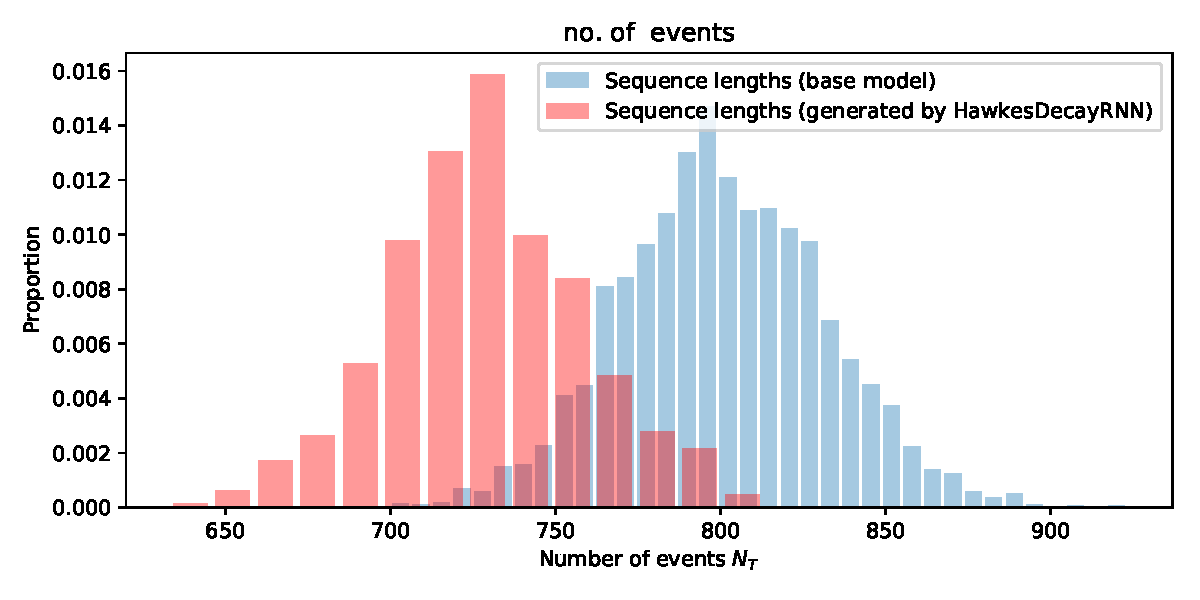
\includegraphics[width=\linewidth]{../results/seq_length_distrib_HawkesDecayRNN-1d-hidden_32-20181205-230630.pdf}
	\caption{Distribution du nombre d'événements. $K=1$ type d'événements. Hawkes vs. Decay-RNN avec $D=32$ neurones cachés. Entraîné sur le jeu de données \autoref{tab:synthHawkesData}.}\label{fig:1DRNNlengthDistrib}
\end{figure}

\begin{figure}[ht]
	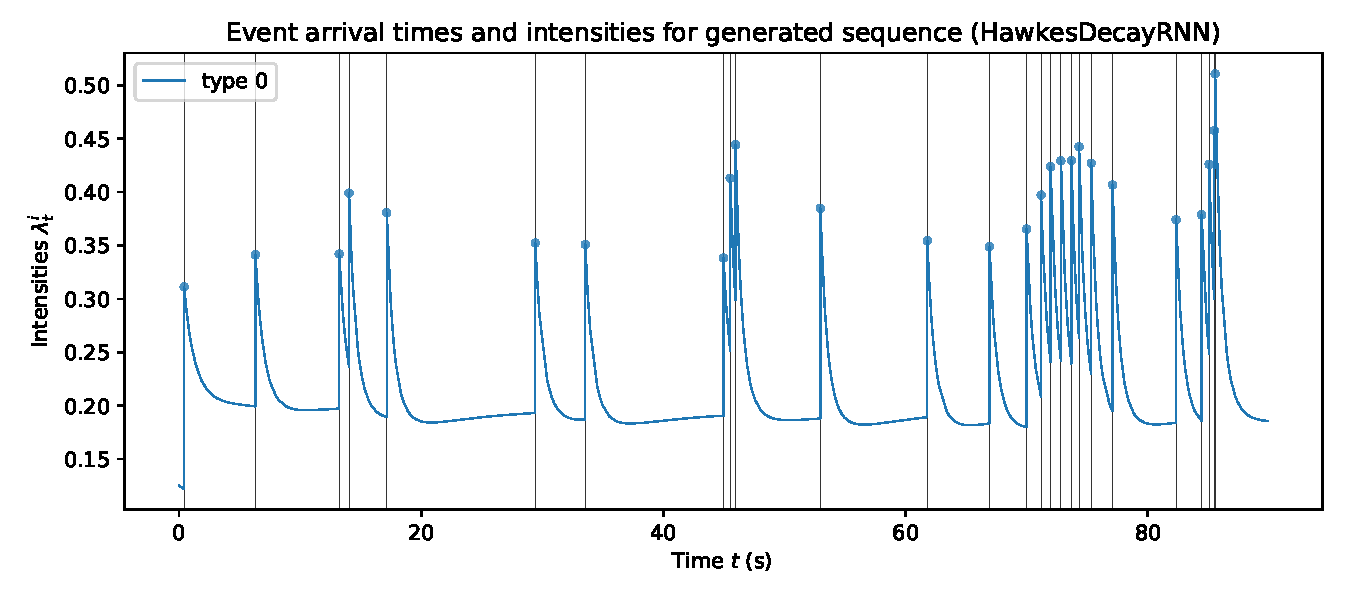
\includegraphics[width=\linewidth]{../results/intensity_HawkesDecayRNN_1d_hidden32_20181205-230630.pdf}
	\caption{Intensité d'un Decay-RNN univarié, entraîné sur les données 1D simulées à partir d'un Hawkes \autoref{tab:synthHawkesData}.}\label{fig:1DRNNintensityPlot}
\end{figure}





\end{document}